\appendix

\chapter{Implementation and Evaluation Addenda}

This appendix chapter provides some more details about finer details about the
implementation and the evaluation that could not fit within the main body of the
dissertation.

\section{The \texttt{Ccode} module}\label{ccode}

The \texttt{Ccode} module stores the OCaml representation of the target C
subset. It is specially chosen to be a subset of C, and only contain the
necessary types to represent the compilation target. There are four main
datatypes in the module, and a quick summary of them is given here:

\begin{itemize}

\item \texttt{Ccode.cident}, for representing identifiers (variable names, macro
    names, function names etc.) in C. This is largely a wrapper over the
    \texttt{Ident.t} type the OCaml compiler uses to represent identifiers,
    which is the string name along with a unique integer ID to disambiguate it
    from other identifiers with the same name.

\item \texttt{Ccode.cexpr}, for representing expressions in C. These include a
    wrapper around \texttt{cident}s, literals, and operations (such as unary
    operations, binary operations, function calls etc.) on other
    \texttt{cexpr}s.

\item \texttt{Ccode.cstatement}, for representing statements in C. Most data
    constructors in this type take a \texttt{cexpr} or a block of other
    \texttt{cstatement}s, and include if statements, while statements, switch
    statements etc. Notably a \texttt{cexpr} can be promoted to a
    \texttt{cstatement}, but not the other way around.

\item \texttt{Ccode.ctype}, for representing types in C. This is an auxiliary
    type used by the casting operator in \texttt{cexpr} and the variable
    declaration statement in \texttt{cstatement}. A more in-depth discussion of
    the types used to represent OCaml values is at \S\ref{value-repr}.

\end{itemize}

In addition, the \texttt{Ccode} module contains some special record types:

\begin{itemize}

\item \texttt{Ccode.cfunc}, which is a record type holding information about the
    return type of the function, the names and types of its arguments, its name,
    its body of code, and its location in the source.

\item \texttt{Ccode.ccode}, which is the record struct that is finally passed
    into \texttt{Cprint} to print the code. It is composed of three lists: the
    block of statements that forms the preamble (which is things like
    \texttt{\#}\texttt{include} directives and global variable declarations),
    the list of functions, and the block of code representing the \texttt{main}
    function.

\end{itemize}

\section{Purpose of \texttt{runtime.h}}

\texttt{runtime.h} is a special header file which needs to be included in the
compilation of the output C file to produce executables from my compiler. It
contains the type declarations mentioned in the implementation chapter, as well
as helper functions and macros used for implementing certain structures and
observability features.

\section{Compilation of basic constructs}\label{basic-constructs}

This section gives an overview of other common basic syntactical structures
in OCaml are compiled into C.

\subsection{Variable scoping differences between C and OCaml}\label{variable-scoping}

In OCaml, each variable is only visible in the body of the expression where it
is bound, whether if that's in a let-binding or a function declaration. This is
in contrast to variable scope in C, where a variable is visible for the entirety
of the rest of the block it is in.

Furthermore, while OCaml does not allow reassignments (of variables, not 
references), it does allow you to bind another variable with the same name:

\begin{lstlisting}[language=Caml]
let x = 1 in
let x = 2 in
print_int x
\end{lstlisting} 

Here the second binding is not reassigning the value of \texttt{x}, rather it's 
creating another variable with the same name. The first variable still exists, 
but it's been shadowed by the second variable making it inaccessible. Note that 
after leaving the body of the second let binding the second variable goes out 
of scope and the first variable is accessible again.

This behaviour can be approximated using C99's block-scoping:

\begin{lstlisting}[language=C]
int x = 1;
{
    int x = 2;
    print_int(x);
}
\end{lstlisting}

Here we see that within the inner block, the second declaration of \texttt{x}
has shadowed the first declaration of \texttt{x}, but the original declaration
of \texttt{x} is still accessible once we leave the inner block (which is also
the behaviour in OCaml). Therefore, we have to pay careful attention to
inserting variable scopes to correctly mirror the shadowing effects in
OCaml.\footnote{Note however we cannot apply this process for variable
    declarations at the top-level, since you cannot insert block-scopes at the
    top level in C. Unfortunately this requires top-level variables to be
renamed.}

\subsection{Meta-notation for compilation}\label{meta-notation}

To describe the compilation process from OCaml expressions into C we use a
C-like meta-notation. Recall from \S\ref{expr-stmt}, each OCaml expression
compiles to a set of C statements and a variable, which the C statements will
have assigned the correct value to after their execution. We therefore denote
the set of C statements an expression \textit{\texttt{e}} compiles into as
\texttt{comp<\textit{e}>}, and the variable it is associated with
\texttt{var<\textit{e}>}. This gives a way of recursively defining the
compilation process by defining \texttt{comp<\textit{e}>} for all possible OCaml
expressions. In the actual compiler, the \texttt{comp<>} functions are
implemented within the \texttt{Ccompile} module, which outputs an equivalent
representation of C using the types in the \texttt{Ccode} module.

As an example, consider the OCaml expression \texttt{\textit{e1} + \textit{e2}}.
We therefore define:

\begin{lstlisting}
comp<$\textit{e1}$ + $\textit{e2}$> :=

declare$\footnotemark$ result;
comp<$\textit{e1}$>; // var<$\textit{e1}$> now contains the correct value
comp<$\textit{e2}$>; // var<$\textit{e2}$> now contains the correct value
result = var<$\textit{e1}$> + var<$\textit{e2}$>;
\end{lstlisting}
\footnotetext{\texttt{declare} here stands for the type of the result of the
expression which is required for variable declarations in C. In general, this
type is not known generally and depends on the specific types of the
subexpressions, so we use \texttt{declare} to stand in for this.}

\texttt{result} refers to some temporary variable name which we assign to this
expression, and we define \texttt{var<\textit{e1} + \textit{e2}> := result}.
Note that this is a common pattern so we will implicitly assume that when
defining the compilation of an expression \texttt{\textit{e}},
\texttt{var<\textit{e}>} will be the variable named \texttt{result} within
\texttt{comp<\textit{e}>}.

\subsection{\texttt{if-then-else} expressions}

OCaml does not have if-statements but if-expressions, which are of the form:

\begin{center}
    \texttt{if \emph{cond} then \emph{A} else \emph{B}}
\end{center}

Using the same notational conventions as in \S\ref{meta-notation}:

\begin{lstlisting}
comp<if $\emph{cond}$ then $\emph{A}$ else $\emph{B}$> :=

declare result;

comp<$\emph{cond}$>;
if (var<$\emph{cond}$>) {
    comp<$\emph{A}$>;
    result = var<$\emph{A}$>;
} else {
    comp<$\emph{B}$>;
    result = var<$\emph{B}$>;
}
\end{lstlisting}

The same trick to propagate results outwards from inner scopes has been 
employed here also.

\subsection{\texttt{while} loops}

While loops are fairly simple in OCaml -- they simply repeatedly evaluate their 
body while the condition evaluates to true. There are no break nor continue 
statements, so there is not a concept of breaking out of a loop early with the 
exception of setting the condition to false. They have the syntax:

\begin{center}
    \texttt{while \emph{cond} do \emph{body} done}
\end{center}

In addition, the overall return value of the loop is \texttt{unit}. The
compilation for them is therefore: 

\begin{lstlisting}
comp<while $\emph{cond}$ do $\emph{body}$ done> :=

comp<$\emph{cond}$>;
declare temp = var<$\emph{cond}$>;
while (temp) {
    comp<$\emph{body}$>;
    comp<$\emph{cond}$>;
}

declare result = make_unit();
\end{lstlisting}

There is one interesting thing of note here: \texttt{\emph{cond}} does need to 
be evaluated twice, once before the loop, and once at the end of the loop. This 
is because the OCaml while loop re-evaluates \texttt{\emph{cond}} at the 
beginning of each iteration, but since OCaml expressions turn into a list of 
statements in C, we cannot fit this re-evaluation into the head of the while 
statement -- instead, a simple and equivalent way around this is to simply 
re-evaluate \texttt{\emph{cond}} at the end of the loop.

\subsection{\texttt{for} loops}

For loops in OCaml are extremely limited. They permit only iteration over a 
fixed range of integers, and also only allow increments in steps of 1. Like 
with while loops, there are no break nor continue statements in OCaml and so 
there is no possibility of exiting a loop early. They have two forms, which are:

\begin{center}
\texttt{for \emph{x} = \emph{start} to \emph{end} do \emph{body} done}\\
\texttt{for \emph{x} = \emph{start} downto \emph{end} do \emph{body} done}\\
\end{center}

These two versions simply iterate up to or down to a certain number 
(inclusive). Since for loops are so incredibly limited, it was decided 
that rather than including for loops in the targeted subset of C, it would be 
easier to also compile these into while loops in C.

\begin{lstlisting}
comp<for $\emph{x}$ = $\emph{start}$ to $\emph{end}$ do $\emph{body}$ done> :=

comp<$\emph{start}$>;
comp<$\emph{end}$>;
int temp1 = var<$\emph{start}$>;
int temp2 = var<$\emph{end}$>;

{
    declare x = temp1;
    while (x <= temp2) {
        comp<$\emph{body}$>;
        x++;
    }
}

declare result = make_unit();
\end{lstlisting}

(Replace \texttt{<=} for \texttt{>=} and \texttt{x++} for \texttt{x--} for 
\texttt{downto}.)

There are a few things about this compilation that warrant elaboration:
\begin{itemize}

\item \texttt{\emph{x}} again needs to be declared in its own scope, as the for
    loop acts as another variable binding site. Thus, the entirety of the for
    loop is wrapped in another block.

\item Note the use of \texttt{temp1} and \texttt{temp2}, which are necessary
    because \texttt{var<\emph{start}>} and \texttt{var<\emph{end}>} may collide
    with the name of the variable \texttt{x} and cause it to be shadowed in the
    inner scope.

\item \texttt{\emph{start}} and \texttt{\emph{end}} are only evaluated once at
    the start of the loop -- after some quick experiments it could be shown that
    OCaml does this as well, i.e. the limits of the iteration range do not
    change while the loop is running.

\item \texttt{\emph{x}} is mutated through the iteration of the loop. This is
    fine, as OCaml for loops only operate on integers, which are copied instead
    of referenced by other constructs in the target subset of C; thus the
    mutation of \texttt{\emph{x}} cannot affect the behaviour of the program.

\end{itemize}

\section{\texttt{Lstaticraise} and \texttt{Lstaticcatch}}

The \texttt{Lambda} IR also has support for static exceptions, which are
exceptions that can only occur across a local scope.\footnote{In contrast to
normal exceptions, which unwind the stack and can jump to an error handler in an
enclosing scope.} This is similar to the behaviour of a \texttt{goto} statement
in C. In particular, the OCaml pattern-match compiler may opt to use a static
exception to avoid duplication of code for certain branches. For example,
consider this match expression:

\begin{lstlisting}[language=Caml]
type color =
  | Red
  | Green
  | Blue
  | Gray of int
  | RGB of int * int * int

match c with
  | Red -> 0
  | Green -> 1
  | Gray x -> 2
  | _ -> 3
\end{lstlisting}

This match expression contains a wildcard expression which matches both 
\texttt{Blue}, which is an integer, and \texttt{RGB}, which is a block. The 
OCaml pattern-match compiler thus compiles it into the following 
\texttt{Lambda} expression:

\begin{lstlisting}
(catch
  (switch* c/xxxx
    case int 0: 0
    case int 1: 1
    case int 2: (exit 1)
    case tag 0: 2
    case tag 1: (exit 1))
  with (1) 3)
\end{lstlisting}

The branches for \texttt{Blue} and \texttt{RGB} have been compiled into a static
exception (the \texttt{exit} expression), to avoid duplicating the expression in
the branch. This behaviour can be emulated with \texttt{goto}s in C.
\texttt{Lstaticcatch} expressions can be compiled simply into an \texttt{if(0)}
and a label, and \texttt{Lstaticraise} expressions are simply compiled into a
\texttt{goto}.

\section{Functions that return other functions}\label{incomplete-funcs}

\S\ref{function-typing} provides a scheme for converting between function types
in OCaml to function types in C, but this conversion doesn't always make sense.
In OCaml, it is possible and often useful to define functions that return other
functions. As a simple example, consider the function:

\begin{lstlisting}[language=Caml]
let f x = (fun y -> x + y)
\end{lstlisting}

The type of \texttt{f} is \texttt{int -> int -> int}, but it's obvious that this
isn't translatable into a C function \texttt{int f(int x, int y)} -- the body of
the function would return a closure, and not an integer.

Since the type of \texttt{f} is known, this is a rather simple problem to fix
via a technique known as eta-expansion, and can be done at the source code
level. Simply add extra parameters to match the number of parameters in the
type, and apply them to the old result of the function.

\begin{lstlisting}[language=Caml]
let f x y = (fun y -> x + y) y
\end{lstlisting}

\section{``Reduced allocations'' mode}\label{reduced-allocs}

In the evaluation we mention that since floating point numbers must be boxed to
be stored in OCaml blocks or polymorphic structures, this makes operations with
them incredibly slow.  It however is still necessary for observability, as
non-integral or pointer types must be tagged with their type within polymorphic
structures so that a debugger is able to infer their types. If we relax this
requirement however, since the OCaml runtime does not otherwise require data to
be tagged with their type, we can store floating point numbers (and other types,
such as closures and strings) directly within OCaml blocks without needing to
make a separate object on the heap.

\begin{figure}
    \centering
    \resizebox{\textwidth}{!}{
        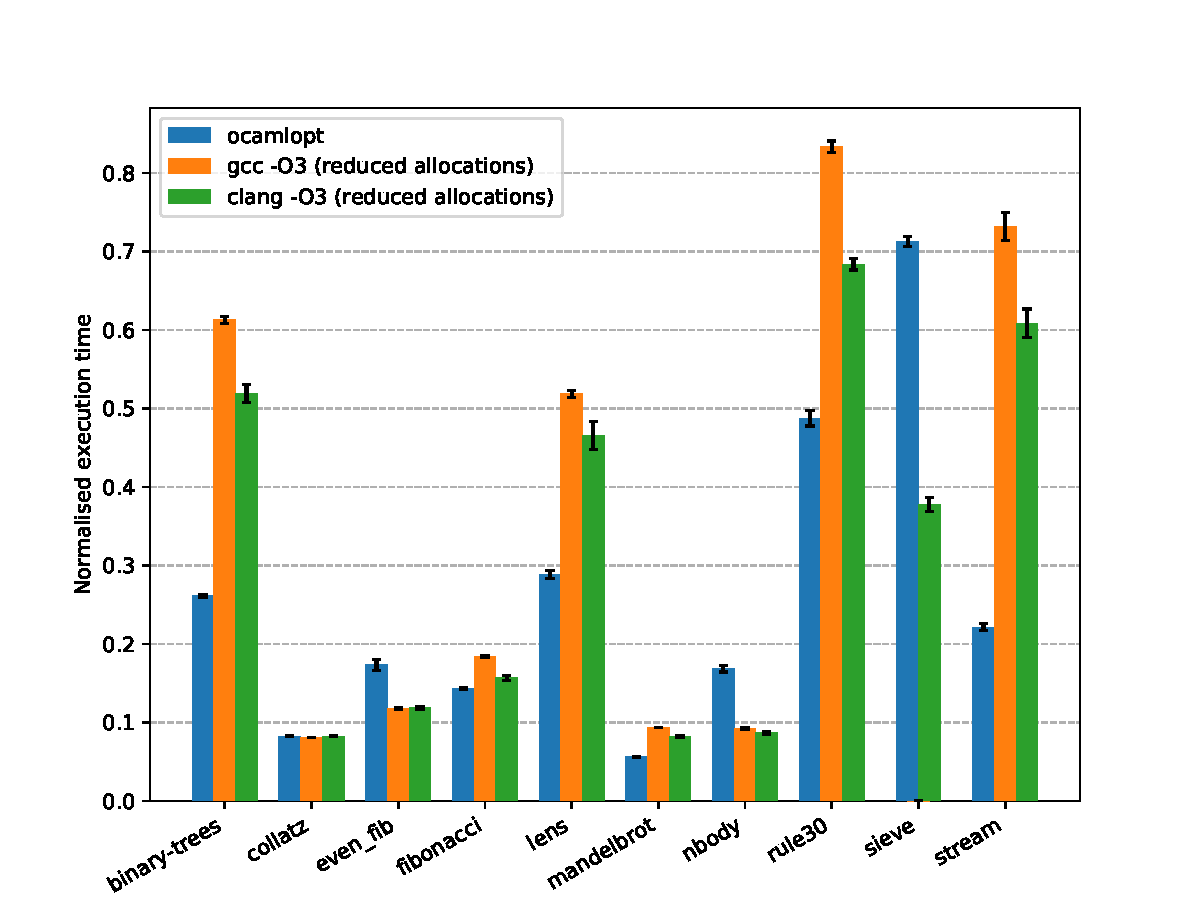
\includegraphics{figs/benchmarks-no-alloc.pdf}
    }

    \caption{Relative speed-up as before in Figure~\ref{fig:raw-benchmarks}.
    While most of the benchmarks do not change much, note that the speed-up
    times for \texttt{mandelbrot} and \texttt{nbody} increase signficantly to
    more closely match the native compiler.}\label{fig:benchmarks-no-alloc}
\end{figure}

I implemented this mode which is accessible via a C compiler flag, and obtained
results which demonstrated far more favourable execution times especially for
the \texttt{mandelbrot} and \texttt{nbody} benchmarks, as can be seen in
Figure~\ref{fig:benchmarks-no-alloc}.

While this change does increase the performance of the code generated by the
compiler, it is worth noting that this means that polymorphic structures are no
longer observable as a debugger cannot determine all the types at runtime, as
well as meaning that functions that require some degree of runtime reflection
such as OCaml's polymorphic comparisons do not function. This means that while
the results provided by this mode are interesting and represent the performance
of the compiler under perhaps a better representation of polymorphic data, the
results represent an interesting side scenario that is not suitable for use
generally. This is possibly fixable with the addition of further run-time
support for polymorphic structures.

\section{Stack overflow}\label{stack-overflow}

Curiously, from the benchmark results in Figure~\ref{fig:raw-benchmarks}, the
executable produced by GCC under all optimisation levels segfaults for the
benchmark \texttt{sieve}. This is in spite of \texttt{sieve} being written in
tail-recursive style, and \texttt{clang} being able to produce a working
executable.

I therefore performed an investigation using M. Godbolt's compiler
explorer,\footnote{\url{https://godbolt.org/}} and narrowed down the offending
code that causes this to the following: 

\begin{lstlisting}[language=C]
typedef union {
    void* ptr;
} val;

void* g(val);

val f(val x) {
    return {.ptr = g(x)};
}
\end{lstlisting}

When compiled with gcc under \texttt{-O3}, this produces the rather confusing
output:

\begin{lstlisting}[basicstyle=\ttfamily\footnotesize,
basewidth={.5em,.3em}, frame=single]
0000000000400590 <f>:
  400590:       48 83 ec 08             sub    rsp,0x8
  400594:       e8 57 ff ff ff          call   4004f0 <g>
  400599:       48 83 c4 08             add    rsp,0x8
  40059d:       c3                      ret    
  40059e:       66 90                   xchg   ax,ax
\end{lstlisting}



Somehow, the cast back into the union type prevents \texttt{gcc} from detecting 
the function call is in tail-call position in this specific case, despite the 
fact that the binary representations for the pointer and the union can be the
same and so no conversion would be required in assembler. This causes the
function to compile to a decrement of the stack pointer, a call to another
function, and then an immediate increment of the stack pointer again, when it
would've been equivalent to a \texttt{jmp} instruction to \texttt{g}.


\chapter{Debug sessions}\label{debug-sessions}

\section{The ``sum'' program}

\begin{lstlisting}[language=Caml, numbers=left, stepnumber=1]
external print_int : int -> unit = "print_int"
external newline : unit -> unit = "newline"

let rec foldl f acc = function
  | x :: xs -> foldl f (f acc x) xs
  | [] -> acc

let sum = foldl (+) 0

let a = sum [1; 2; 3]
let _ = print_int a; newline ()
\end{lstlisting}

\section{GDB session of the ``sum'' program}\label{debug-gdb}

\begin{lstlisting}[basicstyle=\linespread{0.8}\ttfamily\footnotesize, basewidth={.5em,.3em}, frame=single, numbers=left, stepnumber=1, breaklines=true, escapechar=]
GNU gdb (Ubuntu 7.11.1-0ubuntu1~16.5) 7.11.1
Copyright (C) 2016 Free Software Foundation, Inc.
License GPLv3+: GNU GPL version 3 or later <http://gnu.org/licenses/gpl.html>
This is free software: you are free to change and redistribute it.
There is NO WARRANTY, to the extent permitted by law.  Type "show copying"
and "show warranty" for details.
This GDB was configured as "x86_64-linux-gnu".
Type "show configuration" for configuration details.
For bug reporting instructions, please see:
<http://www.gnu.org/software/gdb/bugs/>.
Find the GDB manual and other documentation resources online at:
<http://www.gnu.org/software/gdb/documentation/>.
For help, type "help".
Type "apropos word" to search for commands related to "word"...
Reading symbols from test_gdb...done.
(gdb) source ../../../debug/pprint.py
(gdb) break 4
Breakpoint 1 at 0x400fdc: file test.ml, line 4.
(gdb) run
Starting program: /home/tyler/Code/Coursework/observable-ocaml/tests/observability/sum/test_gdb 

Breakpoint 1, local_func_1222 (f_1207=<closure>, acc_1208=0, param_1211=[0: 1 [0: 2 [0: 3 0]]], closure_obj_1221=<closure>) at test.ml:4
4	let rec foldl f acc = function
(gdb) print acc_1208
$1 = 0
(gdb) step
5	  | x :: xs -> foldl f (f acc x) xs
(gdb) print x_1209
$2 = 1
(gdb) print xs_1210
$3 = [0: 2 [0: 3 0]]
(gdb) continue
Continuing.

Breakpoint 1, local_func_1222 (f_1207=<closure>, acc_1208=1, param_1211=[0: 2 [0: 3 0]], closure_obj_1221=<closure>) at test.ml:4
4	let rec foldl f acc = function
(gdb) print acc_1208
$4 = 1
(gdb) step
5	  | x :: xs -> foldl f (f acc x) xs
(gdb) print x_1209
$5 = 2
(gdb) print xs_1210
$6 = [0: 3 0]
(gdb) continue
Continuing.

Breakpoint 1, local_func_1222 (f_1207=<closure>, acc_1208=3, param_1211=[0: 3 0], closure_obj_1221=<closure>) at test.ml:4
4	let rec foldl f acc = function
(gdb) continue
Continuing.

Breakpoint 1, local_func_1222 (f_1207=<closure>, acc_1208=6, param_1211=0, closure_obj_1221=<closure>) at test.ml:4
4	let rec foldl f acc = function
(gdb) step
6	  | [] -> acc
(gdb) p acc_1208
$7 = 6
(gdb) step
main () at test.ml:11
11	let _ = print_int a; newline ()
(gdb) print a_1213
$8 = 6
(gdb) continue
Continuing.
6
[Inferior 1 (process 32184) exited normally]
(gdb) 
\end{lstlisting}

\section{Ocamldebug session of the ``sum'' program}\label{debug-ocaml}

\begin{lstlisting}[basicstyle=\linespread{0.8}\ttfamily\footnotesize, basewidth={.5em,.3em}, frame=single, numbers=left, stepnumber=1, breaklines=true, escapechar=]
	OCaml Debugger version 4.05.0

(ocd) break @ Test_ocaml 4
Loading program... done.
Breakpoint 1 at 106800: file test_ocaml.ml, line 4, characters 15-81
(ocd) run
Time: 24 - pc: 106832 - module Test_ocaml
Breakpoint: 1
5   | x :: xs -> <|b|>foldl f (f acc x) xs
(ocd) print acc
acc: 'a = <poly>
(ocd) print x
x: 'a = <poly>
(ocd) print xs
xs: 'a list = [<poly>; <poly>]
(ocd) run
Time: 26 - pc: 106832 - module Test_ocaml
Breakpoint: 1
5   | x :: xs -> <|b|>foldl f (f acc x) xs
(ocd) print x
x: 'a = <poly>
(ocd) print xs
xs: 'a list = [<poly>]
(ocd) run
Time: 28 - pc: 106832 - module Test_ocaml
Breakpoint: 1
5   | x :: xs -> <|b|>foldl f (f acc x) xs
(ocd) run
Time: 30 - pc: 106864 - module Test_ocaml
Breakpoint: 1
6   | [] -> <|b|>acc
(ocd) print acc
acc: 'a = <poly>
(ocd) step
Time: 31 - pc: 107040 - module Test_ocaml
10 let a = sum [1; 2; 3]<|a|>
(ocd) next
Time: 47 - pc: 107052 - module Test_ocaml
11 let _ = print_int a<|a|>; newline ()
(ocd) print a
a: int = 6
(ocd) run
6
Time: 79
Program exit.
(ocd)
\end{lstlisting}

\chapter{Project Proposal}

\section*{Introduction and Description of the Work}

This project involves the implementation of a compiler from OCaml to C in such
a way that will allow the resulting executable to be compatible with
DWARF-based debugging tools, such as \texttt{gdb}. This project will use the
existing front-end of the OCaml compiler, but implement a very different
back-end which outputs valid C code that can be compiled using a tool such as
\texttt{gcc} into a debuggable executable. The focus of the compiler is to
optimise for debuggability, or ``observability'', by taking advantage of the
numerous debugging tools available of the C compilation toolchain.

Since the implementation of the full OCaml language is likely too ambitious for
one project, the core project will instead revolve around the implementation of
an interesting subset of OCaml which still provides technically interesting
challenges in its implementation, while extension tasks may extend the
implementation to cover a wider subset of the entire language. An informal
description of said subset will be given in the Substance and Structure
section.

The ``observability'' of the compiler means that where possible the debugger
should behave \emph{as if} it was debugging the OCaml code. This means that the
debugger should consider sections of the compiled machine code to be mapped to
the appropriate lines of code in OCaml. Furthermore, locally bound variables
should be visible from the debugger when execution has reached the relevant
point, meaning that local variables in the C code should mirror the variables
in the OCaml code.

In addition, features such as closures and parametric polymorphism must be
implemented carefully since these features don't have any similar structures in
C for which they could've been mapped to, but also to maintain
``observability'' these must be ``transparent'' to the debugger (for example, a
polymorphic function of the type \verb!'a -> 'a! that has been instantiated as
the type \verb!int -> int! should have this quality be visible from the
debugger). These qualities can be implemented using user-defined commands for
\texttt{gdb}.

The resulting compiler can be evaluated in mainly two contexts. One of these is
a straightforward performance comparison, where a testbed of OCaml programs are
benchmarked across the OCaml native compiler, the OCaml bytecode compiler, and
this project. The other context is the ``observability'' of the compiler; where
programs are stopped at a certain point of their execution and inspected, to
see how much of the internal state of the stack is recoverable. This can be
made in comparison with OCaml's bytecode debugger, \texttt{ocamldebug}.

\section*{Resources Required}

No special resouces are requred that are not open source and freely available
for download.

\section*{Starting Point}

The project, at least initially, will be a fork of the OCaml compiler
obtainable at \url{github.com/ocaml/ocaml} which will take the same front-end
as the existing compiler, but will implement a new back-end for compilation
into C. The work may use other libraries such as \texttt{libffi} and
\texttt{liballocs} but no work of similar scope to the project.

\section*{Substance and Structure of the Project}

The core of the project will be devoted into the implementation of three
incrementally expanding subsets of OCaml. These subsets have been identified
such that each is sufficient to write nontrivial programs in, and features have
been grouped by relation to each other. In this manner work can be easily split
into 3 discrete blocks, each of which will support a new collection of
programs by their completion.

\subsection*{Subset 1}

Subset 1 will be a very simple language with only a limited number of types and
language constructs. The subset will contain only the basic boolean, integer,
floating point and \texttt{unit} types, basic string support (for
input/output), top level function declarations with \texttt{let} and
\texttt{let rec}, which only accept one argument (so as to sidestep the problem
of partial application and closures), \texttt{if}, \texttt{for},
\texttt{while}, \texttt{ref}, as well as basic arithmetic and boolean
operations.

These features were chosen because because they very easily make for a small
minimalist language, and all constructs more or less have direct analogues in C
meaning translation from AST to C code should be fairly easy. Nonetheless, this
small subset is sufficient to write simple programs.

\subsection*{Subset 2}

Subset 2 will focus on the implementation of types and polymorphism, and will
support tuples, lists, parametric polymorphism, algebraic data types, record
types, and \texttt{match} expressions.

The implementation of this subset will require the design of an object
representation for OCaml values. Tuples and record types map easily to structs
in C, while a tagged union can be used for OCaml's ``sum of products'' approach
to algebraic data types. On the first pass, it is quite likely that a naive
``tagged pointer'' type will be used for support for polymorphism, but
extension tasks may experiment with eliminating this need via some method.

The addition of algebraic data types greatly increases the scope of supported
programs, and allows for functions taking multiple arguments (via tuples), list
processing functions, and more complex data structures such as binary trees.

\subsection*{Subset 3}

Subset 3 will finally add treatment of functions as first-class values. This
will include lambdas, lexical closures, and partial application of functions.

The implementation of this subset will require some representation of closures.
While C does support function pointers, it has no lexical closures and as such
a representation where closures are function pointers with an extra
\texttt{void *} pointer that refers to data in the closure is likely to be the
implementation on the first pass. As an extension task, more performant ways of
implementing closures may be investigated, such as potentially dynamically
generating entry points that push the required arguments before jumping to the
body of the function. 

The addition of these features will make higher-order functions representable,
and make available functions such as \texttt{map}, \texttt{filter}, function
composition etc. At this point subset 3 can be considered a fairly minimal but
full-featured functional language.

\subsection*{Evaluation}

Evaluation will require the creation of a small library of test programs. These
programs should be novel and exhibit the full range of language features
supported by the subsets.

Two main methods will then be used to evaluate the compiler. One is
benchmarking performance of the test programs with the existing OCaml native
compiler and the OCaml bytecode compiler. While it is not expected that the C
compiler will match the performance of OCaml official compilers, the goal is to
be within a reasonable margin so that the performance of compiled C code is
comparable. The performance evaluation will be a simple measurement of the
runtime of the compiled executable in relation to the running time of the
executable produced by the OCaml native compiler and the running time of the
interpreter on the bytecode produced by the OCaml bytecode compiler. The test
suite for the performance evaluation will have to be partly written as part of
the project, and partly adapted from the existing OCaml compiler test suite
(\url{github.com/ocaml/ocaml/tree/trunk/testsuite}) or possibly the Computer
Language Benchmarks Game (\url{benchmarksgame.alioth.debian.org}). Since the
compilation source is only a subset of OCaml, not all of the existing test
suite programs will be relevant, and others will require some adaptation for
them to work for the project.

The other method will be the evaluation of the ``observability'' of the C code.
This will take place in two parts: firstly, we can do a test for
``observability'': this will entail a minimum list of requirements, such as
ability to step through OCaml code, ability to print locally bound values,
ability to print types of locally bound variables, and ability to show
instantiation of polymorphic functions into specific types. The second is to
compare the debug outputs of the C code and the OCaml code. The native OCaml
compiler does not allow observation of locally bound values at all, so our C
compiler should beat this easily; although a more interesting comparison would
be with the OCaml bytecode debugger. Breakpoints could be set at randomly
chosen call sites, and the stack traces, visible locals etc.\ could be compared
between \texttt{ocamldebug} and the debug output of the C code.

\subsection*{Extension Tasks}

This project leaves a lot of room for extension tasks. An obvious extension is
to extend the subset to be a more complete subset of OCaml. The next steps
taken would likely be module and exception support, although both are far more
complex features to attempt for implementation in C.

More realistic extension tasks would be changes to the existing code in order
to make it more performant. This would involve improvements to the
implementation of polymorphic functions and closures, as described in their
respective sections prior.

Another plausible extension task is to improve the debug output of OCaml
values. Since C does not have an exact analogue for all OCaml values the debug
output from \texttt{gdb} for example will not look exactly like their OCaml
representation. However, \texttt{gdb} supports the use of custom formatters
written in Python for types and a task to implement a way to generate
formatters to print OCaml values correctly is a suitable extension task.

\section*{Success Criteria}

The following criteria should be achieved at the completion of the project:

\begin{itemize}

    \item A working compiler, that is able to compile the language as described
        in Subset 3 into C code correctly;

    \item An evaluation of performance between the output of the compiler and
        the OCaml native and bytecode compilers;

    \item An evaluation of ``observability'' in the compiled executable with
        tools such as \texttt{gdb}. 

        The evaluation should focus on the following:

        \begin{itemize}

            \item Ability to set breakpoints and step through the compiled
                executable as if it was OCaml code;

            \item Ability to view locally bound variables, and their types,
                although perhaps only as a C ``version'' of the resulting data;

            \item Ability to print more complex data structures, such as ADTs,
                record types and lists;

            \item Similar and comparable output between the debug output and
                the same code running in \texttt{ocamldebug}.

        \end{itemize}

\end{itemize}

Further success criteria, which are not expected to be achieved through the
core project, but interesting as extension tasks may be:

\begin{itemize}

    \item Ability to view the instantiated types of polymorphic functions;

    \item Ability to view data formatted as OCaml values, using specially
        written formatters for \texttt{gdb};

    \item Any number of optimisations on the generated code, resulting in
        better performance benchmarks.

\end{itemize}

\section*{Timetable and Milestones}

\subsection*{20 October --- 3 November}

Initial experiments and reading. Familiarise with the OCaml compiler source
code and obtain typed AST\@. Set up development environment. Write testbed of
evaluation programs so that features can be tested and evaluated immediately
after their implementation.

Milestones: A completed small library of OCaml programs, plus a way of
obtaining the typed AST from the OCaml compiler.

\subsection*{4 November --- 17 November}

Implementation of Subset 1. Evaluation of Subset 1 performance with respect to
the OCaml native and bytecode compilers.

Milestones: A collection of programs now compileable by the Subset 1 compiler,
along with their running times collected in comparison with the OCaml
compilers.

\subsection*{18 November --- 15 December}

Implementation of Subset 2. This is expected to take longer than the
implementation of Subset 1 to take into account that special care needs to be
taken when designing object representations of OCaml values and implementation
of parametric polymorphism. Evaluation of Subset 2 performance with respect to
OCaml compilers.

Milestones: A larger collection of programs now compileable by the Subset 2
compiler, along with their performance results in comparison with the OCaml
compilers.

\subsection*{16 December --- 29 December}

(Two week break for Christmas)

\subsection*{30 December --- 12 January}

Implementation of Subset 3. Evaluation of Subset 3 performance, as well as
comparison between the debug output of the compiled code with
\texttt{ocamldebug}.

Milestones: Completion of core project with the implementation of Subset 3.
Some evaluation results (although perhaps not complete) for the core project.

\subsection*{13 January --- 26 January}

Write up of the Progress Report. Perform any new evaluation tasks that were
missed but become apparent in the write up of the Progress Report. Review the
remainder of the project in context with the existing work and determine which
extension tasks are best to pursue.

Milestones: Completed core project with evaluation, with a completed Progress
Report ready for submission. Entire project reviewed with supervisor and
overseers.

\subsection*{27 January --- 9 February}

Submission of Progress Report. Revise evaluation tasks with feedback from
Progress Report. Prepare Progress Report presentation.

\subsection*{10 February --- 23 February}

Start work on dissertation, as well as the implementation of ways of making the
compiled code more performant. Investigation and use of perhaps \texttt{libffi}
and \texttt{liballocs} to improve performance and observability.

Milestones: The introduction and preparation sections of the dissertation
complete. Improvements on the compiler made, with evaluation results to show
improvements in performance of the compiled output.

\subsection*{24 February --- 9 March}

Start writing the implementation section of dissertation. Implementation of the
generation of custom formatters for \texttt{gdb}, which will make the debug
output easier to read and interpret as OCaml values.

Milestones: Implementation section of the dissertation at least half complete.
Improvements to debug output of debuggers run on the compiled executables.

\subsection*{10 March --- 22 March}

Finish writing implementation section of dissertation. Start evaluation
section. Pick up any further evaluation tasks at this point that become
apparent.

Milestones: Finished implementation section, evaluation section at least half
complete. Revised evaluation tasks in accordance with the write up of the
evaluation section.

\subsection*{23 March --- 5 April}

Finish evaluation and conclusion sections of the dissertation. Deliver draft
dissertation to supervisor and director of studies for feedback. Spend time
working on whatever is in greatest need of attention.

Milestones: Submit a complete draft of the dissertation for review to
supervisor and director of studies.

\subsection*{6 April --- 19 April}

Revise dissertation based on feedback received. Finish any last tasks that
require performing, which are hopefully minor at this point in time. Send
revised drafts for further rounds of review.

\subsection*{20 April ---}

Final adjustments and revisions to dissertation and the body of code. Prepare
for submission of dissertation.

Milestone: Submission of dissertation.

\newpage

\section*{Resource Declaration}

No special resources are required for this project other than those that are
not already available as open source code.

